\documentclass[11pt]{article}
\usepackage{geometry}                % See geometry.pdf to learn the layout options. There are lots.
\geometry{letterpaper}                   % ... or a4paper or a5paper or ... 
%\geometry{landscape}                % Activate for for rotated page geometry
\usepackage[parfill]{parskip}    % Activate to begin paragraphs with an empty line rather than an indent
\usepackage{daves,fancyhdr,natbib,graphicx,dcolumn,amsmath,lastpage,url}
\usepackage{amsmath,amssymb,epstopdf,longtable}
\usepackage{paralist}  % need to properly formulate standard answer blocks
\usepackage[final]{pdfpages}
\DeclareGraphicsRule{.tif}{png}{.png}{`convert #1 `dirname #1`/`basename #1 .tif`.png}
\pagestyle{fancy}
\lhead{CE 3372 Water Systems Design; Exam 2}
\rhead{Name:\_\_\_\_\_\_\_\_\_\_\_\_\_\_\_\_\_\_\_\_\_\_\_\_\_\_\_\_\_\_\_\_\_\_}
\lfoot{REVISION A \small{.}}
\cfoot{}
\rfoot{Page \thepage\ of \pageref{LastPage}}
\renewcommand\headrulewidth{0pt}
\newcommand\tab[1][1cm]{\hspace*{#1}}



\begin{document}
%%%%%%%%%%%%%%%%%%%%%%%%%%%%%%%%%%%
\begingroup
\begin{center}
{\textbf{{ CE 3372 Water Systems Design}  \\ Fall 2016} }
\end{center}
\endgroup

%%%%%%%%%%%%%%%%%%%%%%%%%%%

\begin{enumerate}
%%%%%%%%%%%%%%%%%%%%%%%%%%%%%%%%%%%%%%%%%%%%%%
%%%%%%%% PROBLEM 1 %%%%%%%%%%%%%%%%%%%%%%%%%%%%%%%
%%%%%%%%%%%%%%%%%%%%%%%%%%%%%%%%%%%%%%%%%%%%%%
\item  The hydraulic radius in a conduit containing a flowing liquid is
\begin{enumerate} [(A)]
\item	the mean radius from the center of flow to the wetted side of the conduit
\item	the ratio of the cross-sectional area of the conduit and the wetted perimeter
\item	the ratio of the wetted perimeter and the cross-sectional area of the conduit
\item	the ratio of the cross-sectional area of flow and the wetted perimeter
\end{enumerate}
%%%%%%%%%%%%%%%%%%%%%%%%%%%%%%%%%%%%%%%%%%%%%%
%%%%%%%% PROBLEM 2 %%%%%%%%%%%%%%%%%%%%%%%%%%%%%%%
%%%%%%%%%%%%%%%%%%%%%%%%%%%%%%%%%%%%%%%%%%%%%%
\item The rational runoff coefficient for a $14.81$~acre parcel property is $0.35$.  
The rainfall intensity is $4.56$ inches per hour.  
The peak discharge from this property is anticipated to be about
%standard answer set
\begin{enumerate} [(A)]
\item $22~ft^3/s$
\item $24~ft^3/s$
\item $38~ft^3/s$
\item $70~ft^3/s$
\item $22~ft^3/s$
\item $24~ft^3/s$
\item $38~ft^3/s$
\item $70~ft^3/s$
\end{enumerate}
%\item The rational runoff coefficient for a $300X200$-meter property with a slope of $3$\% is $0.35$.  The rainfall intensity is $116$ mm/hr.  The peak discharge from this property is anticipated to be about
%%standard answer set
%\begin{enumerate} [(A)]
%\item $2200~m^3/hr$
%\item $2400~m^3/hr$
%\item $3800~m^3/hr$
%\item $7000~m^3/hr$
%\end{enumerate}
%======== SOLUTION ===========
% B   Apply Rational Runoff Formula (in SI units)
% NCEES pp 159
%=============================
%
\item  A storm sewer (reinforced concrete pipe) is 400-feet long and 30-inches in diameter.  The sewer flows partially full (not-surcharged) between a personnel access shaft (invert elevation $101.00$ feet) and a lift station sump (invert elevation $100.00$ feet).  Assuming Manning's roughness coefficient is $0.013$ for all flow depths, the sewer capacity is about
%standard answer set
\begin{enumerate} [(A)]
\item  $4.2$ cfs
\item  $9.8$ cfs
\item  $20.5$ cfs
\item  $32.6$ cfs
\item $22~ft^3/s$
\item $24~ft^3/s$
\item $38~ft^3/s$
\item $70~ft^3/s$
\end{enumerate}
%%%%%%%%%%%%%%%%%%%%%%%%%%%%%%%%%%%%%%%%%%%%%%
%%%%%%%% PROBLEM 3 BEGIN %%%%%%%%%%%%%%%%%%%%%%%%%%%
%%%%%%%%%%%%%%%%%%%%%%%%%%%%%%%%%%%%%%%%%%%%%%
%====== SOLUTION ==========================
% C  use Manning's equation for full pipe flow
%  NCEES pp 160-161
%==========================================
%=======================================================================
\clearpage
\item The storm sewer in the question above is flowing at $\frac{3}{4}$ full.  What is the discharge in the sewer?
%standard answer set
\begin{enumerate} [(A)]
\item  $3.6$ cfs
\item  $8.1$ cfs
\item  $12.5$ cfs
\item  $18.1$ cfs
\item $22~ft^3/s$
\item $24~ft^3/s$
\item $38~ft^3/s$
\item $70~ft^3/s$
\end{enumerate}
%%%%%%%%%%%%%%%%%%%%%%%%%%%%%%%%%%%%%%%%%%%%%%
%%%%%%%% PROBLEM 4 DONE %%%%%%%%%%%%%%%%%%%%%%%%%%%
%%%%%%%%%%%%%%%%%%%%%%%%%%%%%%%%%%%%%%%%%%%%%%
\item  A pipe with a diameter of $2.4$ meters is depicted in Figure \ref{fig:CircularSewerToo}.   The pipe is flowing partially full.

\begin{figure}[h!] %  figure placement: here, top, bottom, or page
\centering
   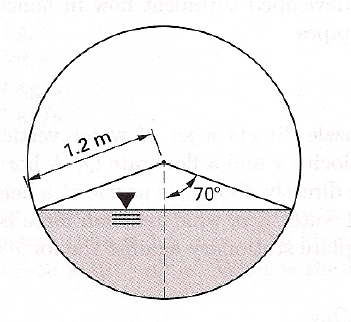
\includegraphics[width=1.9in]{CircularSewerToo.jpg}
   \caption{Circular channel flowing partially full.}
   \label{fig:CircularSewerToo} 
\end{figure}

What is the hydraulic radius of flow in the circular section?
%standard answer set
\begin{enumerate} [(A)]
\item $0.44$ m
\item $0.88$ m
\item $1.30$ m
\item $1.80$ m
\item $0.44$ m
\item $0.88$ m
\item $1.30$ m
\item $1.80$ m
\end{enumerate}
~\clearpage
14. A smooth concrete channel is depicted in Figure \ref{fig:TriangleChannel}.  The channel's dimensionless slope in the direction of flow is $0.005$.  If the flow width at the surface is $2$-meter, what is the flow rate in the channel using the Hazen-Williams friction formula?

\begin{figure}[h!] %  figure placement: here, top, bottom, or page
\centering
   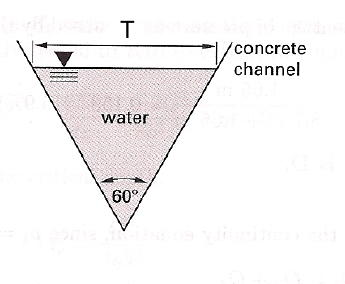
\includegraphics[width=2.2in]{TriangleChannel.jpg}
   \caption{Triangular channel.}
   \label{fig:TriangleChannel} 
\end{figure}

%standard answer set
\begin{enumerate} [(A)]
\item $0.80~ m^3/sec$
\item $1.30~ m^3/sec$
\item $1.45~ m^3/sec$
\item $2.20~ m^3/sec$
\item $22~ft^3/s$
\item $24~ft^3/s$
\item $38~ft^3/s$
\item $70~ft^3/s$
\end{enumerate}
~\newline
%%%%%%%%%%%%%%%%%%%%%%%%%%%%%%%%%%%%%%%%%%%%%%
%%%%%%%% PROBLEM 4 BEGIN %%%%%%%%%%%%%%%%%%%%%%%%%%%
%%%%%%%%%%%%%%%%%%%%%%%%%%%%%%%%%%%%%%%%%%%%%%
\item A 24-inch diameter sewer pipe, with Manning's n of $0.015$ is laid on slope $S_0 =0.01$ as shown in Figure \ref{fig:PipeOnSlope}.    

\begin{figure}[h!] %  figure placement: here, top, bottom, or page
\centering
   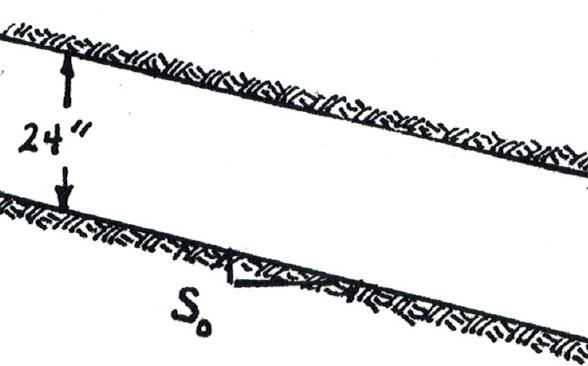
\includegraphics[width=2in]{PipeOnSlope.jpg}
   \caption{Sewer pipe sketch}
   \label{fig:PipeOnSlope} 
\end{figure}
Equation \ref{eqn:CircleDepthArea} is the depth-area equation  and Equation \ref{eqn:CircleWettedPerimeter} is the depth-perimeter equation for a circular conduit where the flow area is $A$, the flow depth is $y$, the diameter is $D$.
and the wetted perimeter is $P_w$.  Use Manning's equation and Equations \ref{eqn:CircleDepthArea} and \ref{eqn:CircleWettedPerimeter}  to complete Table \ref{tab:SewerPipes}.
\begin{equation}
A = \frac{D^2}{4} \{ [cos^{-1}(1-\frac{2y}{D})] - [sin(cos^{-1}(1-\frac{2y}{D}))] \times [cos(cos^{-1}(1-\frac{2y}{D}))] \}
\label{eqn:CircleDepthArea}
\end{equation}

\begin{equation}
P_w = D \times cos^{-1}(1-\frac{2y}{D})
\label{eqn:CircleWettedPerimeter} 
\end{equation}

% Requires the booktabs if the memoir class is not being used
\begin{table}[htbp]
   \centering
   \caption{Depth-Area, Depth-Perimeter, Depth-Hyd. Radius, and Discharge for Circular Sewer}
   \begin{tabular}{p{1in}p{1in}p{1in}p{1in}p{1in}}
   ~ & ~ & ~  & ~ & ~ \\
$y$ ($ft$)~~& $A$ ($ft^2$) & $P_w$ ($ft$) & $R_h$ ($ft$) & $Q$ ($ft^3/sec$) \\
\hline
\hline
~ & ~ & ~  & ~ & ~ \\
1.00 & ~ & ~  & ~ & ~ \\
~& ~ & ~  & ~ & ~ \\
\hline
~ & ~ & ~  & ~ & ~ \\
2.00 & ~ & ~  & ~ & ~ \\
~ & ~ & ~  & ~ & ~ \\
\hline
   \end{tabular}
   \label{tab:SewerPipes}
\end{table}
\clearpage
%%%%%%%%%%%%%%%%%%%%%%%%%%%%%%%%%%%%%%%%%%%%%%%%%%%%%%%%%
\item Figure \ref{fig:SewerPipeMatchFlowline} is a sketch of a $24$ inch line with Manning's n of $0.015$, laid on a slope of $0.01$, connecting to a $48$ inch line (also at $0.01$) at a junction box.   The flowlines (invert elevations) match at the junction box.  The downstream boundary conditions cause the flow depth in the $48$ line to be $12$ inches deep.

\begin{enumerate}[a)]
\item What is the likely flow depth in the $24$ inch line (at the junction box)? \\~\\
\item What is the discharge in the $24$ inch line, assuming normal flow at the flow depth in the junction box? \\~\\
\item What is the discharge in the $24$ inch line, assuming normal flow, when the pipe ($24$ inch) is full? \\~\\
\item What is the unused flow capacity in the $24$ inch line? \\~\\
\end{enumerate}

\begin{figure}[h!] %  figure placement: here, top, bottom, or page
\centering
   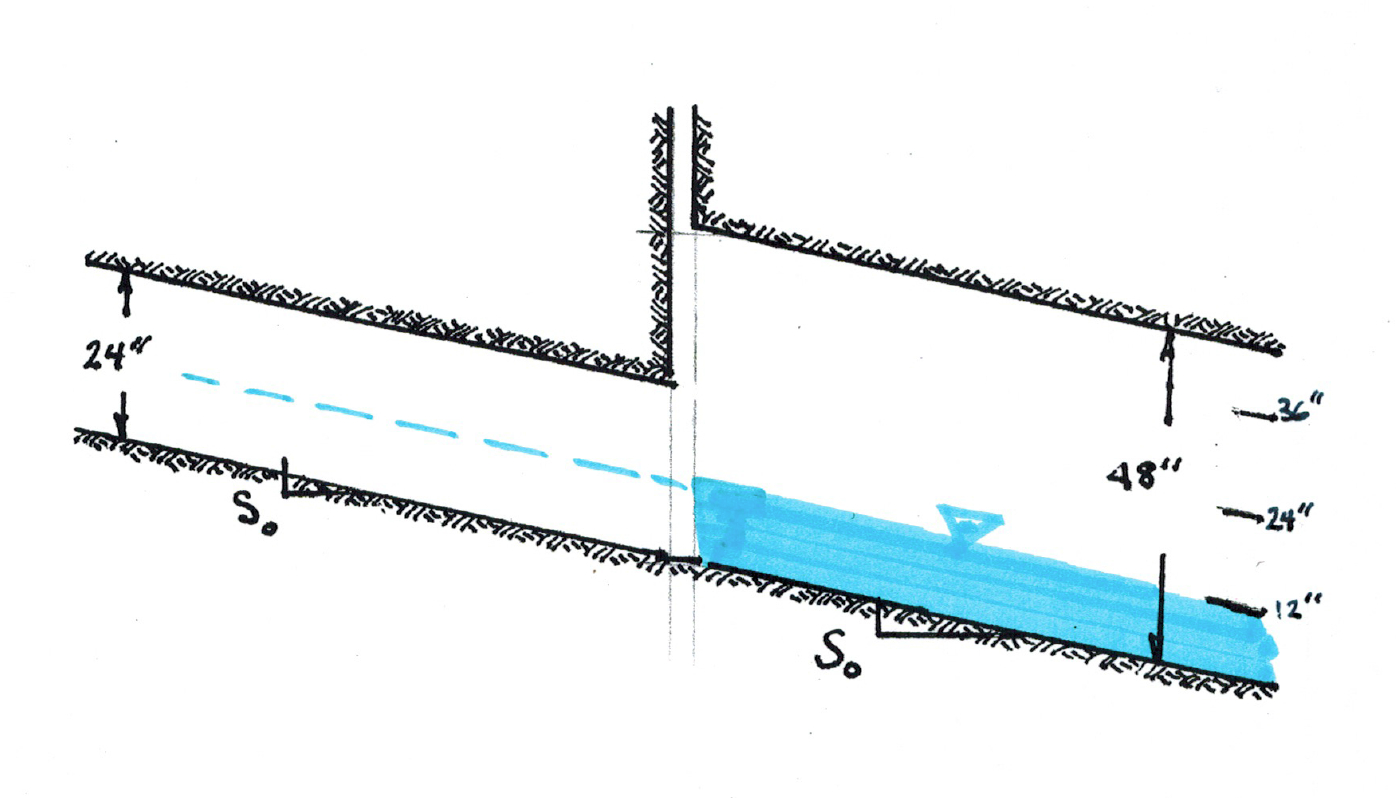
\includegraphics[width=5in]{SewerPipeMatchFlowline.jpg}
   \caption{Sewer pipes connected at a junction box.  Matching flow line elevations.}
   \label{fig:SewerPipeMatchFlowline} 
\end{figure}
\clearpage
%%%%%%%%%%%%%%%%%%%%%%%%%%%%%%%%%%%%%%%%%%%%%%%%%%%%%%%%%
\item Figure \ref{fig:SewerPipeMatchSoffit} is a sketch of a $24$ inch line with Manning's n of $0.015$, laid on a slope of $0.01$, connecting to a $48$ inch line (also at $0.01$) at a junction box.   The soffit(crown) elevations match at the junction box.  The downstream boundary conditions cause the flow depth in the $48$ line to be $36$ inches deep.

\begin{enumerate}[a)]
\item What is the likely flow depth in the $24$ inch line (at the junction box)? \\~\\
\item What is the discharge in the $24$ inch line, assuming normal flow at the flow depth in the junction box? \\~\\
\item What is the discharge in the $24$ inch line, assuming normal flow, when the pipe ($24$ inch) is full? \\~\\
\item What is the unused flow capacity in the $24$ inch line? \\~\\
\end{enumerate}

\begin{figure}[h!] %  figure placement: here, top, bottom, or page
\centering
   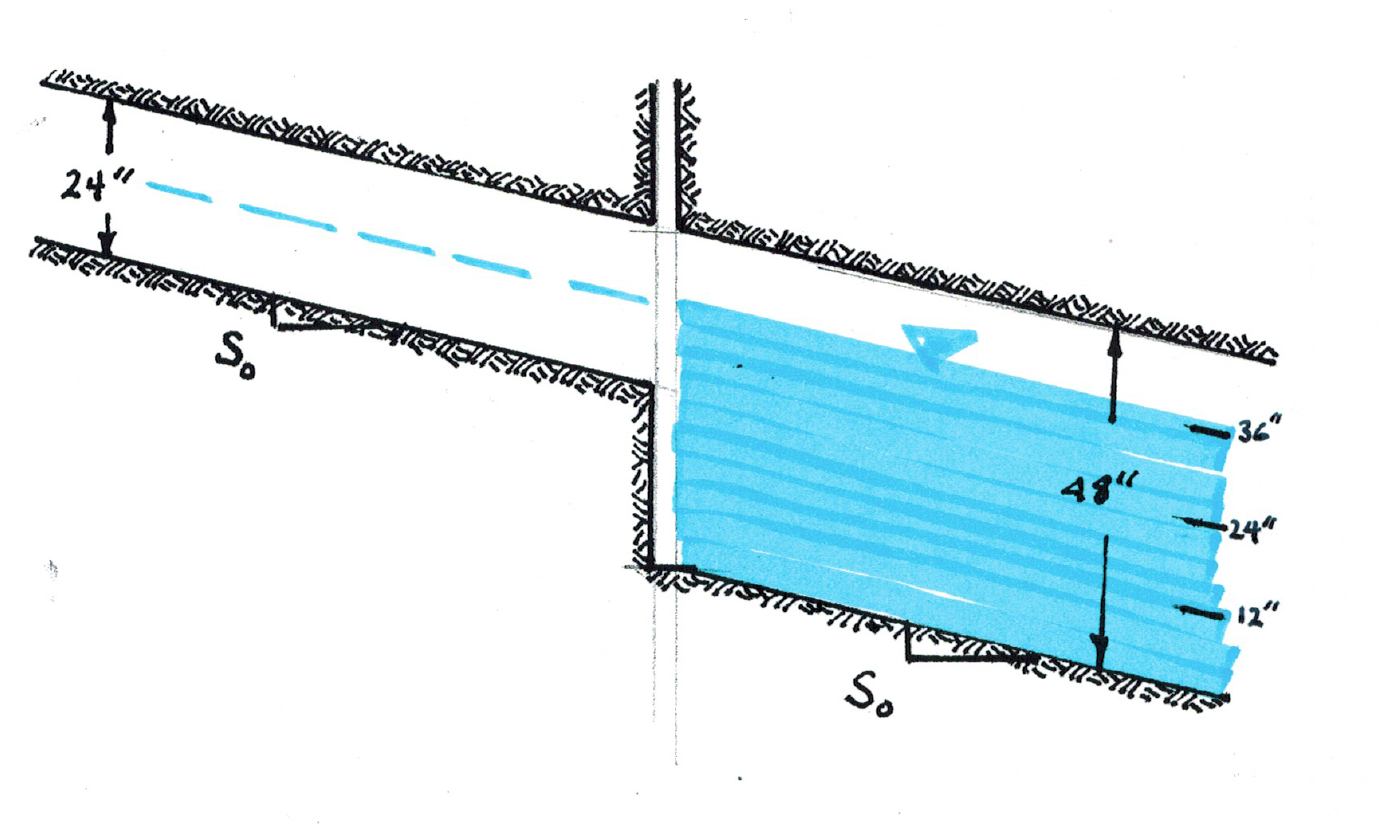
\includegraphics[width=5in]{SewerPipeMatchSoffit.jpg}
   \caption{Sewer pipes connected at a junction box.  Matching soffit elevations.}
   \label{fig:SewerPipeMatchSoffit} 
\end{figure}
\clearpage
%%%%%%%%%%%%%%%%%%%%%%%%%%%%%%%%%%%%%%%%%%%%%%%%%%%%%%%%%
\item Figure \ref{fig:SewerPipeMatchFlowlineDeep} is a sketch of a $24$ inch line with Manning's n of $0.015$, laid on a slope of $0.01$, connecting to a $48$ inch line (also at $0.01$) at a junction box.   The soffit(crown) elevations match at the junction box.  The downstream boundary conditions cause the flow depth in the $48$ line to be $36$ inches deep.

\begin{enumerate}[a)]
\item What is the likely flow depth in the $24$ inch line (at the junction box)? \\~\\
\item What is the discharge in the $24$ inch line, assuming normal flow at the flow depth in the junction box? \\~\\
\item What is the discharge in the $24$ inch line, assuming normal flow, when the pipe ($24$ inch) is full? \\~\\
\item What is the unused flow capacity in the $24$ inch line? \\~\\
\end{enumerate}
\begin{figure}[h!] %  figure placement: here, top, bottom, or page
\centering
   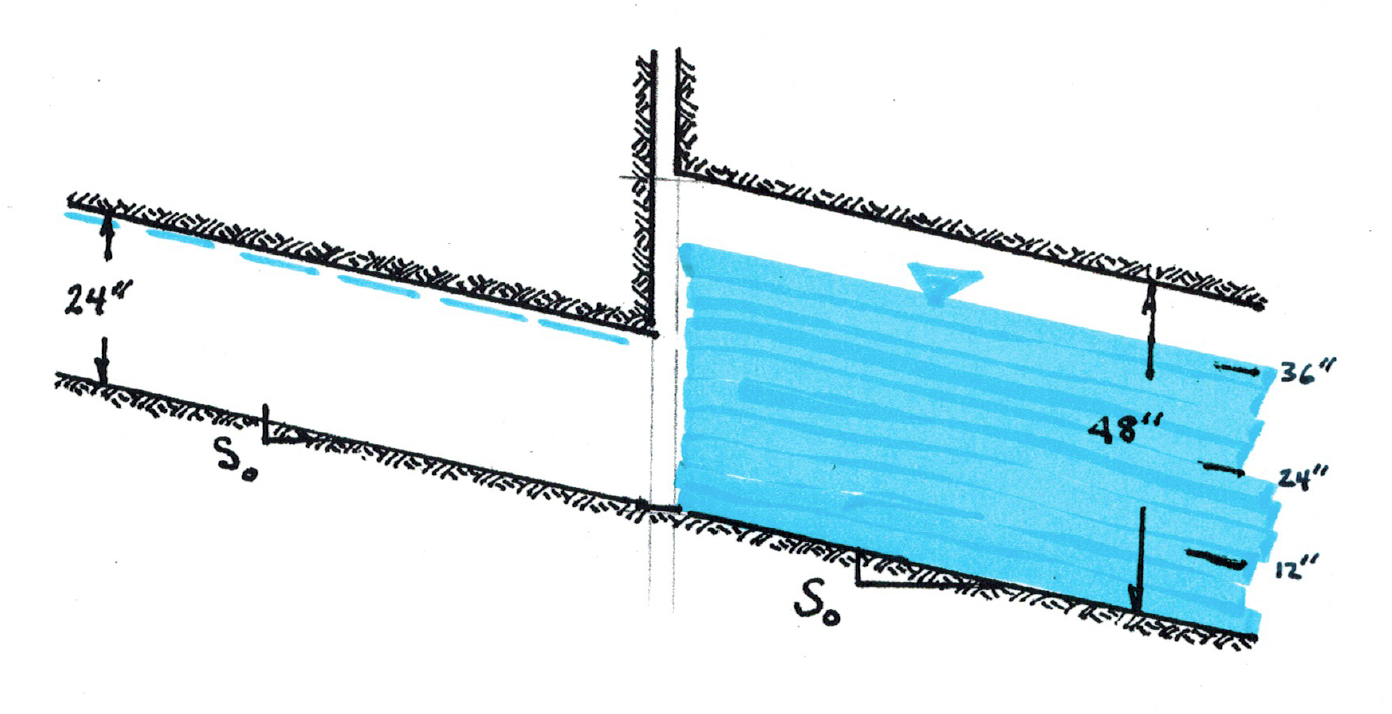
\includegraphics[width=5in]{SewerPipeMatchFlowlineDeep.jpg}
   \caption{Sewer pipes connected at a junction box.  Matching flow line elevations.}
   \label{fig:SewerPipeMatchFlowlineDeep} 
\end{figure}
\clearpage


~\clearpage


%%%%%%%%%%%%%%%%%%%%%%%%%%%%%%%%%%%%%%%%%%%%%%
%%%%%%%% PROBLEM 5 BEGIN %%%%%%%%%%%%%%%%%%%%%%%%%%%
%%%%%%%%%%%%%%%%%%%%%%%%%%%%%%%%%%%%%%%%%%%%%%
%%%%%%%%%%%%%%%%%%%%%%%%%%%%%%%%%%%%%%%%%%%%%%
%%%%%%%% PROBLEM 5 DONE %%%%%%%%%%%%%%%%%%%%%%%%%%%
%%%%%%%%%%%%%%%%%%%%%%%%%%%%%%%%%%%%%%%%%%%%%%




%%%%%%%%%%%%%%%%%%%%%%%%%%%%%%%%%%%%%%%%%%%%%%
%%%%%%%% PROBLEM 2 BEGIN %%%%%%%%%%%%%%%%%%%%%%%%%%%
%%%%%%%%%%%%%%%%%%%%%%%%%%%%%%%%%%%%%%%%%%%%%%
\item A circular, 60-inch diameter, reinforced concrete sewer pipe ($n = 0.013$ )carries 50 MGD of wastewater to a lift station wet well.   Average slope along the flow path is 1.0\%.
%about 50 MGD%
\begin{enumerate} 
\item	Sketch the cross section, indicate the pipe diameter.
~\\
~\\
~\\
~\\
~\\
~\\
~\\
~\\
~\\
~\\
~\\
~\\
~\\
~\\
\item For the conditions in the problem statement, what is the flow rate in cubic feet per second?
~\\
~\\
\item What is the diameter of the pipe, in feet?
~\\
~\\


\item Use Manning's equation ($ Q = \frac{1.49}{n} A R^{(2/3)} S^{(1/2)} $) and determine the \textbf{pipe-full} discharge in cubic feet per second?
~\\
~\\
~\\
~\\
~\\
~\\
\clearpage
\item What is the pipe-full discharge ($Q_{f}$) in million gallons per day (MGD)?
~\\
~\\
~\\
\item Compute the ratio of actual flow ($\frac{Q}{Q_{f}}$) to full pipe flow.
~\\
~\\
~\\
\item What is the ratio of depth of actual flow to full flow ($\frac{d}{D}$) using the hydraulic element chart in Figure \ref{fig:hydraulic-elements}?  Use the highlighted curve.
~\\
~\\
~\\
\begin{figure}[ht!] %  figure placement: here, top, bottom, or page
\centering
   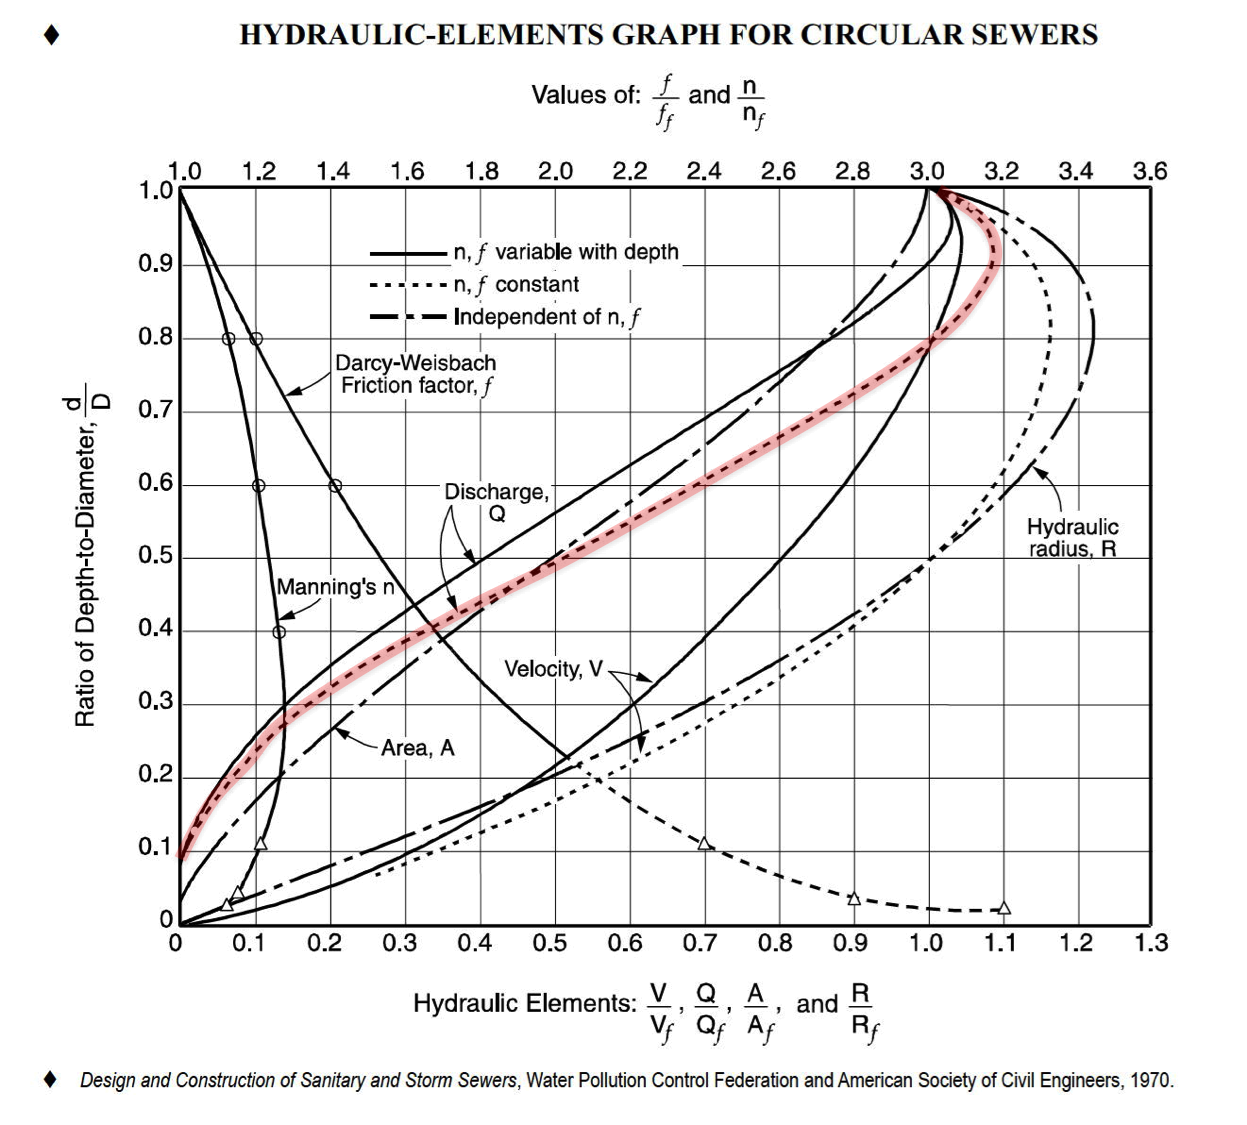
\includegraphics[width=4.5in]{hydraulic-elements.pdf}
   \caption{Hydraulic Elements Chart}
   \label{fig:hydraulic-elements} 
\end{figure}
\clearpage
\item What is the depth of actual flow in feet?
~\\
~\\
~\\
\item What is the depth of actual flow in inches?
~\\
~\\
~\\
\item Modify your sketch to include the water surface position and the approximate flow depth.
~\\
\item Is this portion of sewer close to surcharging?
~\\
\end{enumerate}

\clearpage
%%%%%%%%%%%%%%%%%%%%%%%%%%%%%%%%%%%%%%%%%%%%%%
%%%%%%%% PROBLEM 2 DONE %%%%%%%%%%%%%%%%%%%%%%%%%%%
%%%%%%%%%%%%%%%%%%%%%%%%%%%%%%%%%%%%%%%%%%%%%%



\clearpage
%%%%%%%%%%%%%%%%%%%%%%%%%%%%%%%%%%%%%%%%%%%%%%%
%%%%%%%% EPA PROBLEM BEGIN %%%%%%%%%%%%%%%%%%%%%%%%%%%
%%%%%%%%%%%%%%%%%%%%%%%%%%%%%%%%%%%%%%%%%%%%%%%
\item  An EPA-NET simulation model for a reservoir-pump-network was constructed and operated for four (4) different operational scenarios.   Figure \ref{fig:epa-net-map} is a depiction of the network.   The numbers next to the nodes are Node\_ID values in the reports that follow, and the numbers next to the pipes are the Link\_ID values.  The network is supplied from a reservoir through a booster pump, both are depicted on Figure \ref{fig:epa-net-map}. 

\begin{figure}[h!] %  figure placement: here, top, bottom, or page
\centering
   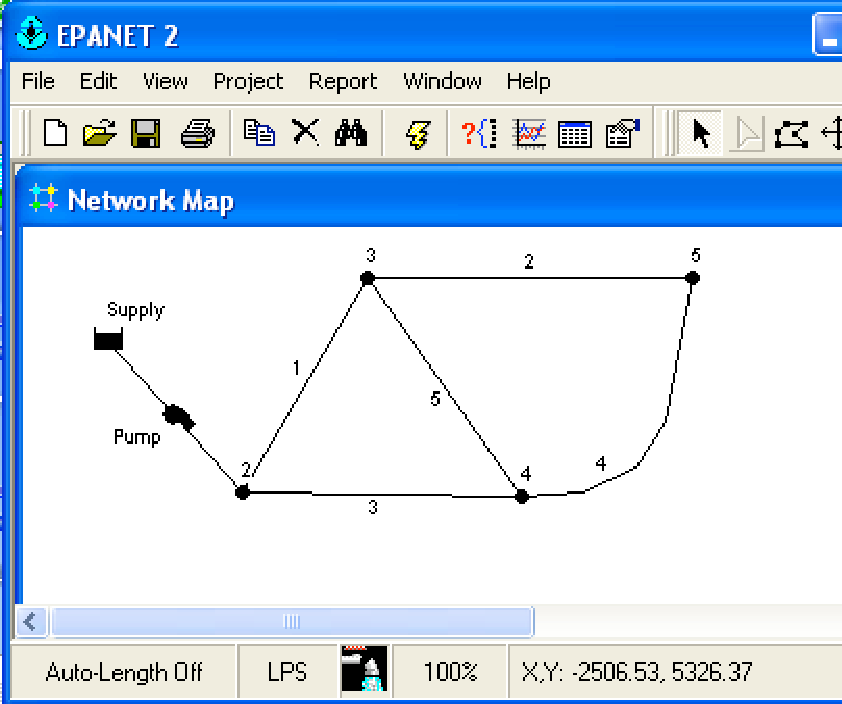
\includegraphics[width=3in]{epa-net-map.pdf}
   \caption{EPA-NET system topology.}
   \label{fig:epa-net-map} 
\end{figure}

Figure \ref{fig:epanet1} is the a portion of the summary report for simulation 1.   
Figure \ref{fig:epanet2} is the a portion of the summary report for simulation 2.  
Figure \ref{fig:epanet3} is the a portion of the summary report for simulation 3.  
Figure \ref{fig:epanet4} is the a portion of the summary report for simulation 4.

These four simulation represent different demand scenarios for the same system.



Interpret these reports, to answer the following questions:

\begin{enumerate}
\item Complete the table below.  $Q_{pump}$ is the discharge in liters-per-second through the pump station, $H_{Supply}$ is the head at the supply reservoir,  $H_{Node2}$ is the head at Node 2, and $\Delta H_{pump}$ is the added head supplied by the pump.
% Requires the booktabs if the memoir class is not being used
\begin{table}[htbp]
   \centering
      \caption{Pump Discharge and Supplied Head}
   \begin{tabular}{p{1in} p{1in} p{1in} p{1in} p{1in} } % Column formatting, @{} suppresses leading/trailing space
Simulation \# & $Q_{pump}$ & $H_{Supply}$ & $H_{Node2}$ & $\Delta H_{pump}$ \\
\hline
\hline
~~1 & ~ &~ & ~ & ~ \\
~ & ~ &~ & ~ & ~ \\
\hline
~~2 & ~ &~ & ~ & ~ \\
~ & ~ &~ & ~ & ~ \\
\hline
~~3 & ~ &~ & ~ & ~\\
~ & ~ &~ & ~ & ~ \\
\hline
~~4 & ~ &~ & ~ & ~ \\
~ & ~ &~ & ~ & ~ \\
\hline
   \end{tabular}
   \label{tab:pump-curve}
\end{table}

\item Complete the table below.  $Q_{pump}$ is the discharge in liters-per-second through the pump station, $\Delta H_{Node 2 -to- 5}$ is head loss in the system from Node 2 to Node 5.
\begin{table}[htbp]
   \centering
      \caption{System Discharge and Head Loss}
   \begin{tabular}{p{1in} p{1in} p{1in} p{1in} p{1in} } % Column formatting, @{} suppresses leading/trailing space
Simulation \# & $Q_{pump}$ & $H_{Node2}$ & $H_{Node5}$ & $\Delta H_{Node 2 -to- 5}$ \\
\hline
\hline
~~1 & ~ &~ & ~ & ~ \\
~ & ~ &~ & ~ & ~ \\
\hline
~~2 & ~ &~ & ~ & ~ \\
~ & ~ &~ & ~ & ~ \\
\hline
~~3 & ~ &~ & ~ & ~\\
~ & ~ &~ & ~ & ~ \\
\hline
~~4 & ~ &~ & ~ & ~ \\
~ & ~ &~ & ~ & ~ \\
\hline
   \end{tabular}
   \label{tab:system-curve}
\end{table}



\item If the pump performance curve has the mathematical structure: ~\\
$H_{pump} = H_{shutoff} - K_{pipe} \times Q^2$, estimate the values of $H_{shutoff}$  and $K_{pipe}$.
\\
\\
\\
\\
\\
\\
\\
\\
\\
\\
\\
\\
\\
\item If the system frictional loss curve has the mathematical structure:
 $H_{pipe}= K_{loss} \times Q^2$, estimate the value of $K_{loss}$

\clearpage
\item What effect would removing the pipe joining nodes 3 and 4 have on the system performance?   Explain your reasoning.
\\
\\
\\
\\
\\
\\
\\
\\
\\
\\
\\
\\
\\
\item Estimate the flow distribution and head losses the the system if the the pipe joining nodes 3 and 4 are removed, and the pipe joining node 4 and 5 is removed if the nodal demands are the same as SIMULATION  2.
\end{enumerate} 

%%% YOUR ON YOUR OWN %%%%%%%%%%%%%%%%%%%%
\begin{figure}[ht!] %  figure placement: here, top, bottom, or page
\centering

\begin{verbatim}
  Page 1                                            10/4/2010 2:27:47 PM
  **********************************************************************
  *                             E P A N E T                            *
  *                     Hydraulic and Water Quality                    *
  *                     Analysis for Pipe Networks                     *
  *                           Version 2.0                              *
  **********************************************************************
  Input File: SIMULATION #1
Link - Node Table:
  ----------------------------------------------------------------------
  Link           Start          End                Length  Diameter
  ID             Node           Node                    m        mm
  ----------------------------------------------------------------------
  1              2              3                    1000       124
  2              3              5                    1000       124
  3              2              4                    1000       124
  4              4              5                    1000       124
  5              3              4                    1400       124
  7              6              2                    #N/A      #N/A Pump
Node Results:
  ----------------------------------------------------------------------
  Node                Demand      Head  Pressure   Quality
  ID                     LPS         m         m          
  ----------------------------------------------------------------------
  2                     0.00     20.00     20.00      0.00
  3                     0.00     20.00     20.00      0.00
  4                     0.00     20.00     20.00      0.00
  5                     0.00     20.00     20.00      0.00
  6                     0.00      0.00      0.00      0.00 Reservoir
Link Results:
  ----------------------------------------------------------------------
  Link                  Flow  VelocityUnit Headloss    Status
  ID                     LPS       m/s      m/km
  ----------------------------------------------------------------------
  1                     0.00      0.00      0.00      Open
  2                     0.00      0.00      0.00      Open
  3                     0.00      0.00      0.00      Open
  4                     0.00      0.00      0.00      Open
  5                     0.00      0.00      0.00      Open
  7                     0.00      0.00    -20.00      Open Pump
  \end{verbatim}
     \caption{EPA-NET Summary Report, Simulation \#1}
   \label{fig:epanet1} 
\end{figure}


\begin{figure}[ht!] %  figure placement: here, top, bottom, or page
\centering
\begin{verbatim}
 Page 1                                            10/4/2010 2:28:15 PM
  **********************************************************************
  *                             E P A N E T                            *
  *                     Hydraulic and Water Quality                    *
  *                     Analysis for Pipe Networks                     *
  *                           Version 2.0                              *
  **********************************************************************
  Input File: SIMULATION 2
  Link - Node Table:
  ----------------------------------------------------------------------
  Link           Start          End                Length  Diameter
  ID             Node           Node                    m        mm
  ----------------------------------------------------------------------
  1              2              3                    1000       124
  2              3              5                    1000       124
  3              2              4                    1000       124
  4              4              5                    1000       124
  5              3              4                    1400       124
  7              6              2                    #N/A      #N/A Pump
  Node Results:
  ----------------------------------------------------------------------
  Node                Demand      Head  Pressure   Quality
  ID                     LPS         m         m          
  ----------------------------------------------------------------------
  2                     0.00     19.28     19.28      0.00
  3                     1.00     19.03     19.03      0.00
  4                     1.00     19.03     19.03      0.00
  5                     1.00     18.99     18.99      0.00
  6                    -3.00      0.00      0.00      0.00 Reservoir                                                              
  Link Results:
  ----------------------------------------------------------------------
  Link                  Flow  VelocityUnit Headloss    Status
  ID                     LPS       m/s      m/km
  ----------------------------------------------------------------------
  1                     1.50      0.12      0.25      Open
  2                     0.50      0.04      0.03      Open
  3                     1.50      0.12      0.25      Open
  4                     0.50      0.04      0.03      Open
  5                     0.00      0.00      0.00      Open
  7                     3.00      0.00    -19.28      Open Pump
  \end{verbatim}
     \caption{EPA-NET Summary Report, Simulation \#2}
   \label{fig:epanet2} 
\end{figure}

\begin{figure}[ht!] %  figure placement: here, top, bottom, or page
\centering

\begin{verbatim}
   Page 1                                            10/4/2010 2:29:00 PM
  **********************************************************************
  *                             E P A N E T                            *
  *                     Hydraulic and Water Quality                    *
  *                     Analysis for Pipe Networks                     *
  *                           Version 2.0                              *
  **********************************************************************
  Input File: SIMULATION 4
 Link - Node Table:
  ----------------------------------------------------------------------
  Link           Start          End                Length  Diameter
  ID             Node           Node                    m        mm
  ----------------------------------------------------------------------
  1              2              3                    1000       124
  2              3              5                    1000       124
  3              2              4                    1000       124
  4              4              5                    1000       124
  5              3              4                    1400       124
  7              6              2                    #N/A      #N/A Pump
Node Results:
  ----------------------------------------------------------------------
  Node                Demand      Head  Pressure   Quality
  ID                     LPS         m         m          
  ----------------------------------------------------------------------
  2                     0.00     17.12     17.12      0.00
  3                     2.00     16.16     16.16      0.00
  4                     2.00     16.16     16.16      0.00
  5                     2.00     16.04     16.04      0.00
  6                    -6.00      0.00      0.00      0.00 Reservoir
Link Results:
  ----------------------------------------------------------------------
  Link                  Flow  VelocityUnit Headloss    Status
  ID                     LPS       m/s      m/km
  ----------------------------------------------------------------------
  1                     3.00      0.25      0.96      Open
  2                     1.00      0.08      0.12      Open
  3                     3.00      0.25      0.96      Open
  4                     1.00      0.08      0.12      Open
  5                     0.00      0.00      0.00      Open
  7                     6.00      0.00    -17.12      Open Pump
  \end{verbatim}
     \caption{EPA-NET Summary Report, Simulation \#3}
   \label{fig:epanet3} 
\end{figure}

\begin{figure}[ht!] %  figure placement: here, top, bottom, or page
\centering

\begin{verbatim}
  Page 1                                            10/4/2010 2:29:46 PM
  **********************************************************************
  *                             E P A N E T                            *
  *                     Hydraulic and Water Quality                    *
  *                     Analysis for Pipe Networks                     *
  *                           Version 2.0                              *
  **********************************************************************
  Input File: SIMULATION 3
Link - Node Table:
  ----------------------------------------------------------------------
  Link           Start          End                Length  Diameter
  ID             Node           Node                    m        mm
  ----------------------------------------------------------------------
  1              2              3                    1000       124
  2              3              5                    1000       124
  3              2              4                    1000       124
  4              4              5                    1000       124
  5              3              4                    1400       124
  7              6              2                    #N/A      #N/A Pump
Node Results:
  ----------------------------------------------------------------------
  Node                Demand      Head  Pressure   Quality
  ID                     LPS         m         m          
  ----------------------------------------------------------------------
  2                     0.00     13.52     13.52      0.00
  3                     3.00     11.40     11.40      0.00
  4                     3.00     11.40     11.40      0.00
  5                     3.00     11.15     11.15      0.00
  6                    -9.00      0.00      0.00      0.00 Reservoir
 Link Results:
  ----------------------------------------------------------------------
  Link                  Flow  VelocityUnit Headloss    Status
  ID                     LPS       m/s      m/km
  ----------------------------------------------------------------------
  1                     4.50      0.37      2.12      Open
  2                     1.50      0.12      0.25      Open
  3                     4.50      0.37      2.12      Open
  4                     1.50      0.12      0.25      Open
  5                     0.00      0.00      0.00      Open
  7                     9.00      0.00    -13.52      Open Pump
  \end{verbatim}
     \caption{EPA-NET Summary Report, Simulation \#4}
   \label{fig:epanet4} 
\end{figure}
\clearpage


\end{enumerate}

\end{document}  




